\subsection{Ca sử dụng điền khảo sát sở thích}
\vspace{0.5cm}


\noindent 
\begin{tabularx}{\linewidth}{| l | X |} 
\hline 
\textbf{Mô tả} & Người dùng cập nhật thông tin về sở thích du lịch của bản thân để sử dụng dịch vụ gợi ý trong ứng dụng. \\ 
\hline 
\textbf{Luồng cơ bản} & 1. Người dùng đăng ký tài khoản mới \newline
                       2. Ứng dụng hiển thị các form lựa chọn lần lượt theo loại hình du lịch, giá tiền,... \newline
                       3. Người dùng chọn các loại hình du lịch theo sở thích. \newline
                       5. Người dùng chọn khoảng giá du lịch phù hợp với bản thân. \newline
                       6. Người dùng nhấn nút hoàn tất để hoàn thành quá trình. \newline
                       7. Hệ thống điều hướng người dùng đến trang chủ của ứng dụng. \\
\hline 
\textbf{Tiền điều kiện} & Người dùng đăng ký tài khoản thành công và chưa hoàn thành điền khảo sát sở thích. \\
\hline 
\textbf{Hậu điều kiện} & Thông tin sở thích được lưu lại trong cơ sở dữ liệu. \\

\hline 
\textbf{Yêu cầu phi chức năng} & Hệ thống xử lý cập nhật không quá 1s \\ 
\hline 
\end{tabularx}

\vspace{0.8cm}

\noindent 
\begin{tabular}{| c | c |}
    \hline
    \textbf{Biểu đồ hoạt động} & \textbf{Quan hệ} \\ 
    \hline
    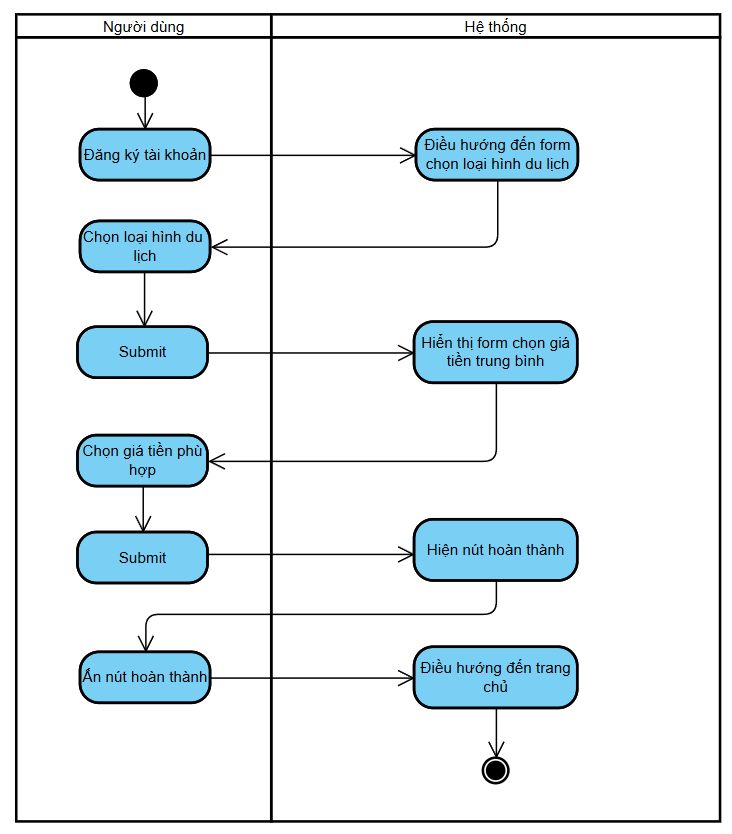
\includegraphics[width=0.5\linewidth]{figures/c3/3-3-3-ad.png} 
    & 
    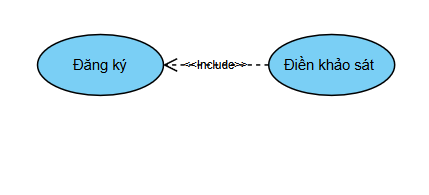
\includegraphics[width=0.45\linewidth]{figures/c3/3-3-3-rd.png} \\ 
    \hline
\end{tabular}



\begin{figure}[H]
    \centering  
    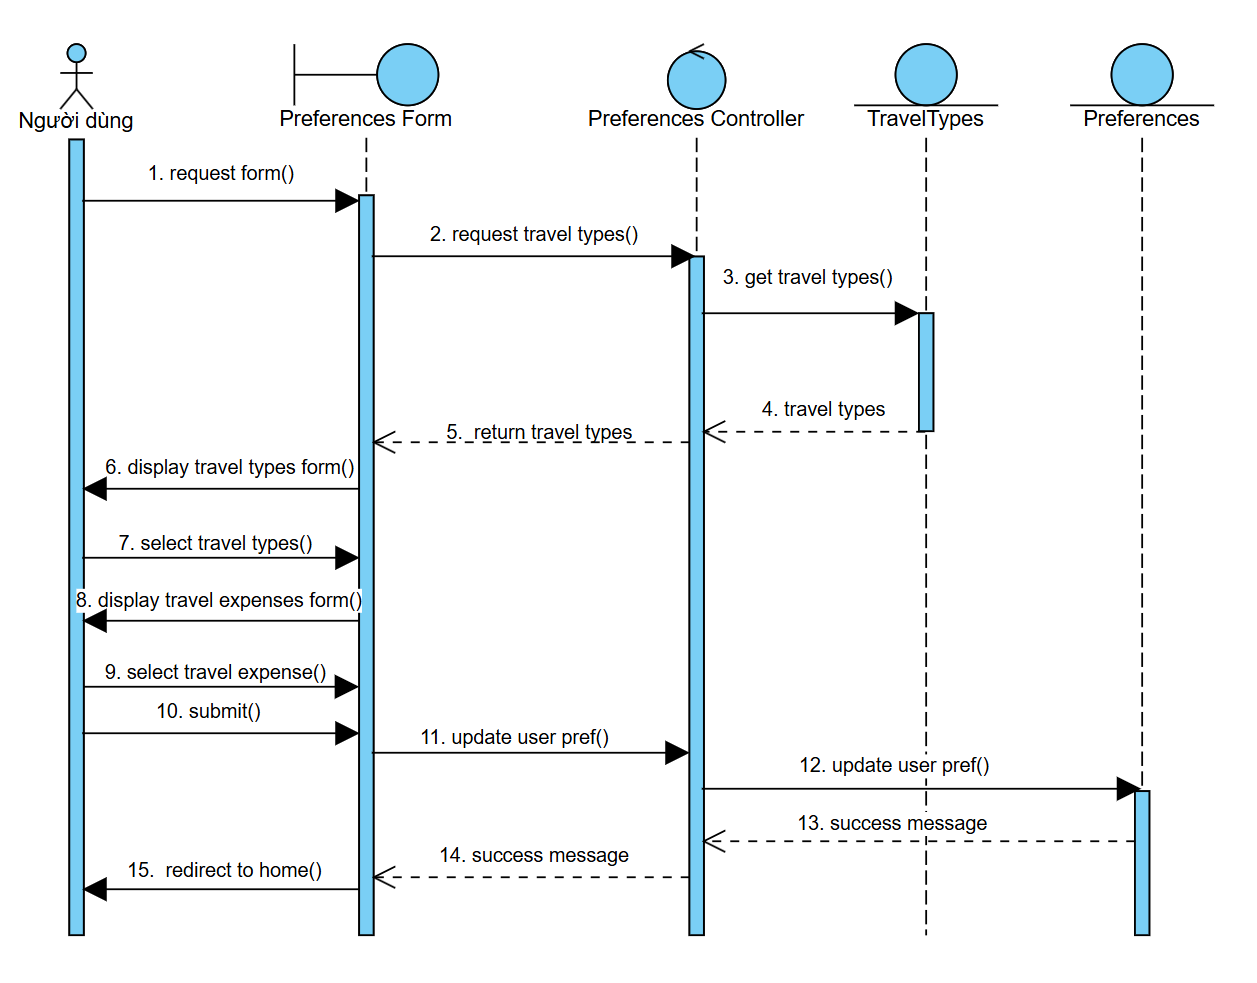
\includegraphics[width=1\textwidth]{figures/c3/3-3-3-sd.png}
    \caption{Biểu đồ tuần tự ca sử dụng điền khảo sát sở thích.}
    \label{fig:3-3-3-sequence-diagram}
\end{figure}